\chapter{Symbolic Block Linear Algebra}
\label{chp:matrix}


In mathematics literature, it is common practice to represent matrices as being broken up into blocks or sub-matrices.
For example if $A$, $B$, $C$ and $D$ are matrices given by:
\begin{equation*}
	A = \begin{bmatrix} 
		A_{1,1} & \ldots & A_{1,m} \\
		\vdots & & \vdots \\
		A_{n,1} & \ldots & A_{n,m}
	\end{bmatrix}
	\;\;\;
	B = \begin{bmatrix} 
		B_{1,1} & \ldots & B_{1,q} \\
		\vdots & & \vdots \\
		B_{n,1} & \ldots & B_{n,q}
	\end{bmatrix}	
	\;\;\;
	C = \begin{bmatrix} 
		C_{1,1} & \ldots & C_{1,m} \\
		\vdots & & \vdots \\
		C_{r,1} & \ldots & C_{r,m}
	\end{bmatrix}
	\;\;\;
	D = \begin{bmatrix} 
		D_{1,1} & \ldots & D_{1,q} \\
		\vdots & & \vdots \\
		D_{r,1} & \ldots & D_{r,q}
	\end{bmatrix}			
\end{equation*}
Where, critically, $A$ and $C$ have the same width (namely $m$) as do $B$ and $D$ (width $q$).
Additionally, $A$ and $B$ have the same height (in this case $n$), as do $C$ and $D$ (height $r$).
Then they can be ``glued'' together into a single  $\boldsymbol{(2 \times 2)}$ \textbf{block matrix} $M$.
Notationally, we write these matrices as elements of $M$ but we \emph{interpret} $M$ as a sort of concatenation of the
sub-matrices.
\begin{equation}
	M= \left[
		\begin{array}{c|c}
			A & B \\
			\hline
			C & D \\
		\end{array}
	\right] = \left[
		\begin{array}{ccc|ccc}
			A_{1,1} & \ldots &A_{1,m} & B_{1,1} & \ldots & B_{1,q} \\
			\vdots & & \vdots & \vdots & & \vdots \\
			A_{n, 1} & \ldots & A_{n, m} & B_{n,1} & \ldots & B_{n,q} \\
			\hline
			C_{1, 1} & \ldots & C_{1, m} & D_{1,1} & \ldots & D_{1,q} \\
			\vdots & & \vdots & \vdots & & \vdots \\
			C_{r,1} & \ldots & C_{r,m} & D_{r,1} & \ldots & D_{r,q} \\
		\end{array}
	\right]
\end{equation}


So $M$ is actually a $(n+r) \times (m+q)$ matrix but we write it as a $2 \times 2$ \emph{block} matrix.
Within an individual block, there is a one-to-one correspondence from the entries of $M$ to the entries of a sub-matrix 
(shifted by some offset).
In the above example, elements of $B$ would have an offset of $(0,m)$ since $B_{i,j}$ corresponds with $M_{i+0, j+m}$.


There is no reason to stop at combining 4 matrices into a $2 \times 2$ block matrix.
We can take a set of matrices $A_{i,j}$ and combine them into an $\boldsymbol{(n\times m)}$ \textbf{block matrix}:
\begin{equation*}
	M = \left[ \begin{array}{c|c|c|c}
		A_{1,1} & A_{1,2} &\ldots & A_{1,m} \\
		\hline
		A_{2,1} & A_{2,2} & \ldots & A_{2,m} \\
		\hline
		\vdots & \vdots & & \vdots \\
		\hline
		A_{n,1} & A_{n,2} & \ldots & A_{n,m}

	\end{array}\right]
\end{equation*}


In the $2\times 2$ case, we enforced that for example the height of $A$ was the same as the height of $B$.
Similarly, here it is an important condition that these partitions are divided by \emph{unbroken} horizontal and vertical lines.
Formally, for each sub-matrix $A_{i,j}$ in $M$ then $A_{i,j}$ is a $s_i \times t_j$ matrix for strictly positive integer sequences $\{s_i\}_{i=1}^n$ and $\{t_j\}_{j=1}^m$ common to all sub-matrices.
As before we interpret the block matrix as a concatenation of its sub-matrices.
Thus $M$ is a $n\times m$ block matrix but a $\left( \sum_{i=1}^n s_i \right) \times \left( \sum_{j=1}^m t_j \right)$
block matrix.


Clearly block matrices are at the very least a convenient notation but they also have considerable practical applications as well.
For example when multiplying large matrices, block matrices can be used to improve cache complexity \cite{lam1991cache}.
Additionally, in some cases, when a sub-matrices are known to have a nice properties, many optimizations can arise.
For example to invert what is known as a \emph{block diagonal matrix}, one can invert each block individually:
\begin{equation}
	\begin{bmatrix}
		A_1 & 0 & \ldots & 0 \\
		0 & A_2 & \ddots & \vdots \\
		\vdots & \ddots & \ddots & 0 \\
		0 & \ldots & 0 & A_n \\
	\end{bmatrix}^{-1}
	=
	\begin{bmatrix}
		{A_1}^{-1} & 0 & \ldots & 0 \\
		0 & {A_2}^{-1} & \ddots & \vdots \\
		\vdots & \ddots & \ddots & 0 \\
		0 & \ldots & 0 & {A_n}^{-1} \\
	\end{bmatrix}
\end{equation}


\begin{figure}[ht] 
	\begin{subfigure}[b]{0.24\textwidth}
		\caption{}
		\begin{equation*}
			\left[ \begin{array}{c|c}
				\; & \; \\
				\hline
				& \\
			\end{array}\right]
		\end{equation*}
	\end{subfigure}
	\begin{subfigure}[b]{0.24\textwidth}
		\caption{}
		\begin{equation*}
			\left[ \begin{array}{c|c}
				\; & \; \\
				\hline
				* & * \\
				\hline
				& \\
			\end{array}\right]
		\end{equation*}
	\end{subfigure}
	\begin{subfigure}[b]{0.24\textwidth}
		\caption{}
		\begin{equation*}
			\left[ \begin{array}{c|c|c}
				\; & * & \;  \\
				\hline
				\; & * &\; \\
			\end{array}\right]
		\end{equation*}
	\end{subfigure}
	\begin{subfigure}[b]{0.24\textwidth}
		\caption{}
		\begin{equation*}
			\left[ \begin{array}{c|c|c}
				\; & * & \; \\
				\hline
				* & * & * \\
				\hline
				\; & * & \; \\
			\end{array}\right]
		\end{equation*}
	\end{subfigure}
	\caption[Possible block overlaps of $2 \times 2$ block matrices.] {
		The sum of two block matrices each with four blocks leads to 9 possible cases.
		When blocks are exactly the same size, the sum will also be a $2 \times 2$ block matrix (a).
		Otherwise, a $2 \times 3$ (b) \emph{(two possible cases)}, $3 \times 2$ (c) \emph{(two cases)} 
		or $3 \times 3$ (d) \emph{(four cases)} block matrix could arise.
		The starred blocks may sample from different blocks depending on the relative size of operand blocks.
	\label{MatAdditionPermutations}}
\end{figure}

Existing techniques allow for fixed block size but are unsatisfactory when the bounds between blocks are symbolic.
For example, the sum of $2 \times 2$ block matrices, naively leads to 9 possible cases of overlapping regions depending on
the relationship between horizontal and vertical boundaries between blocks.
In this chapter we will show a method using hybrid functions to avoid this case based approach for both addition
and multiplication of matrices.
First we introduce some notation that will be used frequently over the next few chapters.

%%%%%%%%%%%%%%%%%%%%%%%%%%%%%%%%%%%%%%%%%
%
% INTERVALS
%
%%%%%%%%%%%%%%%%%%%%%%%%%%%%%%%%%%%%%%%%%

\section{Oriented Intervals}
\label{sec:OrientedIntervals}

\begin{definition}
	Given a totally ordered set $(X, \leq)$ \emph{(and with an implied strict ordering $<$)}, 
	for any $a,b \in X$, an \textbf{interval between $\boldsymbol{a}$ and $\boldsymbol{b}$} 
	is the set of elements in $X$ between $a$ and $b$, up to inclusion of $a$ and $b$ themselves. 
	Formally:
	\begin{equation} 
	\begin{array}{cc}
		{[a,b]}_X =  \{ x \in X \;|\; a \leq x \leq b \} \\
		{[a,b)}_X =  \{ x \in X \;|\; a \leq x < b \} \\
		{(a,b]}_X =  \{ x \in X \;|\; a < x \leq b \} \\
		{(a,b)}_X =  \{ x \in X \;|\; a < x < b \}
	\end{array} 
	\end{equation}
	When context makes $X$ obvious or the choice of $X$ is irrelevant, we shall omit the subscript.
\end{definition}

It should be noted that when $b$ is less than $a$, $[b,a]$ is the empty set. 
In terms of idempotency, the bounds determine whether or not an interval will be empty.
$[a,a]$ which contains $a$ and all points equivalent to $a$ while $(a,a)$, $(a,a]$, and $[a,a)$ are all empty sets.
As intervals are simply sets, they can naturally be interpreted as hybrid sets.
If $a \leq b \leq c$, for intervals then we have $[a,b) \oplus [b,c) = [a,c)$.
In this case, $\oplus$ seems to behave like concatenation but this is not always true.
If instead we had $a \leq c \leq b$ then $[a,b) \oplus [b,c) = [a,b)$.

\begin{equation*}
	[a,b) \oplus [b,c) =
	\begin{cases}
		[a,c) & a \leq b \leq c \\
		[a,b) & a \leq c \leq b \\
		[b,c) & b \leq a \leq c \\
		\emptyset & \text{otherwise} \\
	\end{cases}
\end{equation*}


One could alternatively write $[a,b)\oplus [b,c) = [\; \min(a,b),\max(b,c) \;)$ but this simply sweeps the problem 
under the rug.
When working with intervals, a case-based approach to consider relative ordering of endpoints easily becomes 
quite cumbersome.
Previously, the $\xi$ function was introduced in \cite{sexton2008abstract} to solve this problem.
Although it solves the problem of cases, it quickly leads to unnecessarily heavy notation.
Instead we introduce oriented intervals which are considerably more readable.
It should be noted that the definitions are equivalent; $\xi(i,y,z)$ and $[\![y,z)\!)$ can be used interchangeably.

\begin{definition}
	We define \textbf{oriented intervals} with $a,b\in X$, where $X$ is a totally ordered set, 
	using hybrid set point-wise subtraction as follows:
	\begin{equation}
		\begin{array}{cc}
			{[\![ a,b )\!)} = [a,b) \ominus [b,a) \\
			{(\!( a,b ]\!]} = (a,b] \ominus (b,a] \\
			{[\![ a,b ]\!]} = [a,b] \ominus (b,a) \\
			{(\!( a,b )\!)} = (a,b) \ominus [b,a]
		\end{array}
	\end{equation}
\end{definition}


For any choice of \emph{distinct} $a$ and $b$, exactly one term will be empty; there can be no ``mixed'' multiplicities from a single oriented interval.
Unlike traditional interviews where $[a,b)$ would be empty if $b < a$,  
the oriented interval $[\![a,b)\!)$ will have elements with negative multiplicity.
Several results follow immediately from this definition.

\begin{theorem} For all $a,b,c$, 
	\begin{equation}
		\begin{array}{cc}
		{[\![a,b)\!)} = \ominus [\![b,a)\!) \\
		{(\!(a,b]\!]} = \ominus (\!(b,a]\!] \\
		{[\![a,b]\!]} = \ominus (\!(a,b)\!) \\
		{(\!(a,b)\!)} = \ominus [\![a,b]\!]
		\end{array}
	\end{equation}
\end{theorem}


We should make a note here how oriented intervals behave when $a=b$.
Like their unoriented analogues, the oriented intervals $[\![ a,a )\!)$ and $(\!( a,a ]\!]$ are still both empty sets.
The interval $[\![a,a]\!]$ still contains points equivalent to $a$ (with multiplicity 1).
However, unlike traditional intervals $(\!(a,a)\!)$ is \emph{not} empty but rather, $(\!(a,a)\!) = \ominus [\![a,a]\!]$ and so contains all points equivalent to $a$ but with a multiplicity of $-1$.
The advantage of using oriented intervals is that now $\oplus$ does behave like concatenation.


\begin{theorem}
	For all $a,b,c$ (regardless of relative ordering),
	\begin{equation}
		[\![ a,b )\!) \oplus [\![ b,c )\!) = [\![ a,c )\!)
	\end{equation}
\end{theorem}
\begin{proof}
	Following from definitions we have:
	\begin{align*}
		[\![a,b)\!) \oplus [\![ b,c )\!)
		& = \left( [a,b) \ominus [b,a) \right) \oplus \left( [b,c) \ominus [c,b) \right)\\
		& = \left( [a,b) \oplus [b,c) \right) \ominus \left( [c,b) \oplus [b,a) \right)
	\end{align*}
	\begin{description}
		\item[Case 1: $a \leq c$] then $[c,a) = \emptyset$ and so $[\![a,c)\!) = [a,c)$. 
		\begin{description}
			\item[Case 1.a: $a \leq b \leq c$] then $[c,b) = [b,a) = \emptyset$ and $[a,b) \oplus [b,c) = [a,c)$
			\item[Case 1.b: $b \leq a \leq c$] then $[b,c) \ominus [b,a) = [b,a) \oplus [a,c) \ominus [b,a) = [a,c)$
			\item[Case 1.c: $a \leq c \leq b$] then $[a,b) \ominus [c,b) = ([a,c) \oplus [c,b)) \ominus [c,b) = [a,c)$
		\end{description}
		\item[Case 2: $c < a$] then $[a,c) = \emptyset$ and so $[\![a,c)\!) = \ominus [c,a)$. 
		\begin{description}
			\item[Case 2.a: $c \leq b \leq a$] 
				then $[a,b) = [b,c) = \emptyset$ and $\ominus[c,b) \ominus [b,a) = \ominus [c,a)$
			\item[Case 2.b: $b \leq c \leq a$] 
				then $\ominus [b,a) \oplus [b,c) = \ominus([b,c) \oplus [c,a)) \oplus [b,c) = \ominus[c,a)$
			\item[Case 2.c: $c \leq a \leq b$] 
				then $\ominus [c,b) \oplus [a,b) = \ominus([c,a) \oplus [a,b)) \oplus [a,b) = \ominus[c,a)$
		\end{description}
	\end{description}
\end{proof}


This sort of reasoning is routine but a constant annoyance when dealing with intervals 
and is exactly the reason we want to be working with oriented intervals.
But now that the above work is done, we can use oriented intervals 
and not concern ourselves with the relative ordering of points.
Many similar formulations such as $[\![ a,b ]\!] \oplus (\!( b,c )\!) = [\![a,c)\!)$ or $(\!(a,b)\!) \oplus [\![b,c)\!) = (\!(a,c)\!)$ 
are also valid for any ordering of $a,b,c$ by an identical argument. 



%%%%%%%%%%%%%%%%%%%%%%%%%%%%%%%%%%%%%%%%%
%
% VECTORS
%
%%%%%%%%%%%%%%%%%%%%%%%%%%%%%%%%%%%%%%%%%

\section{Vector Addition}
Addition for partitioned vectors and $2 \times 2$ matrices using hybrid functions has already been considered in \cite{sexton2008abstract, carette2010}.
The method is nearly identical to that of adding piecewise functions.
In fact, one could think of both as simply addition of piecewise functions over a subset of 
$\mathbb{N}$ and $\mathbb{N} \times \mathbb{N}$ respectively.
However it will provide a good example of oriented intervals in use and as an introduction to multiplication of 
symbolic block matrices.


First we will consider the addition of two $n$-dimensional vectors.
Addition of two vectors: $U= (u_1, u_2, \ldots u_n$ and $V = (v_1, v_2, \ldots, v_n)$ is itself an $n$ dimensional vector 
defined as:
\begin{equation}
	U+V = (u_1+v_1, \; u_2+v_2, \ldots, u_n+v_n)
\end{equation}


In particular, we would like to consider the addition of vectors $U$ and $V$ which are each partitioned into two intervals,
$[1,k]$ and $(k,n]$ as well as $[1,\ell]$ and $(\ell, n]$.
Over each interval, taking the value of different functions, as in:
\begin{align}
	U &= [ u_1, u_2, \ldots, u_{k}, u'_1, u'_2, \ldots, u_{n-k} ] \\
	V &= [ v_1, v_2, \ldots, v_{\ell}, v'_1, v'_2, \ldots, v_{n-\ell} ]
\end{align}


These can be written more concisely as hybrid functions over intervals. 
Using intervals, these vectors can be represented by hybrid functions over their indices.
For example
\begin{align}
	U &= (i \mapsto u_i)^{[\![1, k]\!]} \oplus (i \mapsto u_{i-k})^{(\!(k,n]\!]} \\
	V &= (i \mapsto v_i)^{[\![1, \ell]\!]} \oplus (i \mapsto v_{i-\ell})^{(\!(\ell,n]\!]}
\end{align}
Although for clarity and succinctness we will use $(u_i)$ instead of $(i \mapsto u_i)$.
\begin{align}
	U &= (u_i)^{[\![1, k]\!]} \oplus (u_{i-k})^{(\!(k,n]\!]} \\
	V &= (v_i)^{[\![1, \ell]\!]} \oplus v_{i-\ell})^{(\!(\ell,n]\!]}
\end{align}


To add $U$ and $V$
\begin{align}
	U + V
	&= \left( (u_i)^{[\![1, k]\!]} \oplus (u'_{i-k})^{(\!(k,n]\!]} \right) 
		+
		\left( (v_i)^{[\![1, \ell]\!]} \oplus (v'_{i-\ell})^{(\!(\ell,n]\!]} \right) \\
	&= \left( (u_i)^{[\![1, k]\!]} \oplus (u'_{i-k})^{(\!(k,\ell]\!]} \oplus (u'_{i-k})^{(\!(\ell,n]\!]} \right) 
		+
		\left( (v_i)^{[\![1, k]\!]} \oplus (v_i)^{(\!(k, \ell]\!]} \oplus (v'_{i-\ell})^{(\!(\ell,n]\!]} \right) \\
	&= \R[+] \left( (u_i + v_i)^{[\![1, k]\!]} 
		\oplus (u'_{i-k} + v_i)^{(\!(k,\ell]\!]} 
		\oplus (u'_{i-k}+v'_{i-\ell})^{(\!(\ell,n]\!]} \right)
\end{align}


The choice to partition $[\![1,n]\!]$ into $[\![1,k]\!] \oplus (\!(k,\ell]\!] \oplus (\!(\ell, n]\!]$ is only one common refinement.
We can just as easily use $[\![1,\ell]\!] \oplus (\!(\ell, k]\!] \oplus (\!(k, n]\!]$ to get the equivalent expression:
\begin{equation}
	U + V = \R[+] \left( (u_i + v_i)^{[\![1, \ell]\!]} 
		\oplus (u_{i} + v'_{i-\ell})^{(\!(\ell,k]\!]} 
		\oplus (u'_{i-k}+v'_{i-\ell})^{(\!(k,n]\!]} \right)
\end{equation}


We must be careful while evaluating these expressions to not forget that $(u'_{i-k} + v_i)$ 
is actually shorthand for the function:
\begin{equation*}
	(u'_{i-k} + v_i) = (i \mapsto u'_{i-k}) + (i \mapsto v_i) = (i \mapsto u'_{i-k} + v_i)
\end{equation*}
As a function, it may not be evaluable over the entire range implied in a given term.
The same lambda-lifting trick of using pseudo-functions as in the previous section easily solves this.


For example, consider the concrete example where $n=5$, $k=4$ and $\ell = 1$ so that
$U = [ u_1, u_2, u_3, u_4, u'_1 ]$ and
$V = [ v_1, v'_1, v'_2, v'_3, v'_4 ]$.
We will also only assume that the functions $u_i, u'_i, v_i$ and $v'_i$ are defined only on the intervals in which they 
appear (e.g. $u_5$ is undefined, as is $v'_1$).
Then we have:
\begin{equation*}
	U + V = (u_i + v_i)^{[\![1,4]\!]} \oplus (u'_{i-4} + v_i)^{(\!(4,1]\!]} \oplus (u'_{i-4} + v'_{i-1})^{(\!(1,5]\!]}
\end{equation*}

None of the individual sub-terms cannot be evaluated directly.
In the first term, $v_i$ is not totally defined over the interval $[\![1,4]\!]$.
In the third term, on the interval $(\!(1,5]\!]$, $u'_{i-4}$ would even evaluated on negative indices.
However, these un-evaluable terms also appear in the middle term however the interval $(\!(4,1]\!]$ is a negatively oriented
 interval and the offending points cancel exactly as in the previous chapter.
\begin{align*}
	U + V
		&= (u_i + v_i)^{[\![1,1]\!] \oplus (\!(1,4]\!]} 
			\oplus (u'_{i-4} + v_i)^{\ominus(\!(1,4]\!]} 
			\oplus (u'_{i-4} + v'_{i-1})^{(\!(1,4]\!] \oplus (\!(4,5]\!]}\\
		&= (u_i + v_i)^{[\![1,1]\!]} 
			\oplus \left((u_i + v_i) - (u'_{i-4} + v_i) + (u'_{i-4} + v'_{i-1})\right)^{[\![1,4]\!]} 
			\oplus (u'_{i-4} + v'_{i-1})^{(\!(4,5]\!]} \\ 
		&= (u_i + v_i)^{[\![1,1]\!]} 
			\oplus (u_i + v'_{i-1})^{(\!(1,4]\!]} 
			\oplus (u'_{i-4} + v'_{i-1})^{(\!(4,5]\!]}
\end{align*}

%%%%%%%%%%%%%%%%%%%%%%%%%%%%%%%%%%%%%%%%%
%
% N-CUBES
%
%%%%%%%%%%%%%%%%%%%%%%%%%%%%%%%%%%%%%%%%%

\section{Higher Dimension Intervals}

Oriented intervals work perfectly well when we are only dealing with the indices of a vector. 
However, we are more interested in the rectangular blocks of a matrix.
We can move from 1-dimensional intervals to 2-dimensional blocks using the Cartesian product
\begin{definition}
	Let $X = \hset{ x_1^{m_1}, ... , x_k^{m_k} }$ and $Y= \hset{ y_1^{n_1}, ... , y_\ell^{n_\ell} }$ be hybrid sets
	over sets $S$ and $T$
	We define the \textbf{Cartesian product of hybrid sets $\boldsymbol{X}$ and $\boldsymbol{Y}$}, to be a hybrid set
	over $S \times T$ and denoted with $\times$ operator as
	\begin{equation}
		X \times Y = \hset{ (x, y)^{m \cdot n} \; : \; x \in^m X, y \in^n Y }
	 \end{equation}
\end{definition}


If $[\![a,b]\!]$ and $[\![c,d]\!]$ are both positively oriented intervals in $\mathbb{R}$ then their Cartesian product 
$[\![a,b]\!] \times [\![c,d]\!]$ is shown in Figure 4.1 is clearly a two dimensional rectangle in $\mathbb{R}^2$.
If one of $[\![a,b]\!]$ or $[\![c,d]\!]$ were negatively oriented then we would have a negatively oriented rectangle.
If both were negative, then the signs will cancel and the Cartesian product will be \emph{positively} oriented.


\begin{figure}[ht] 
	\centering 
	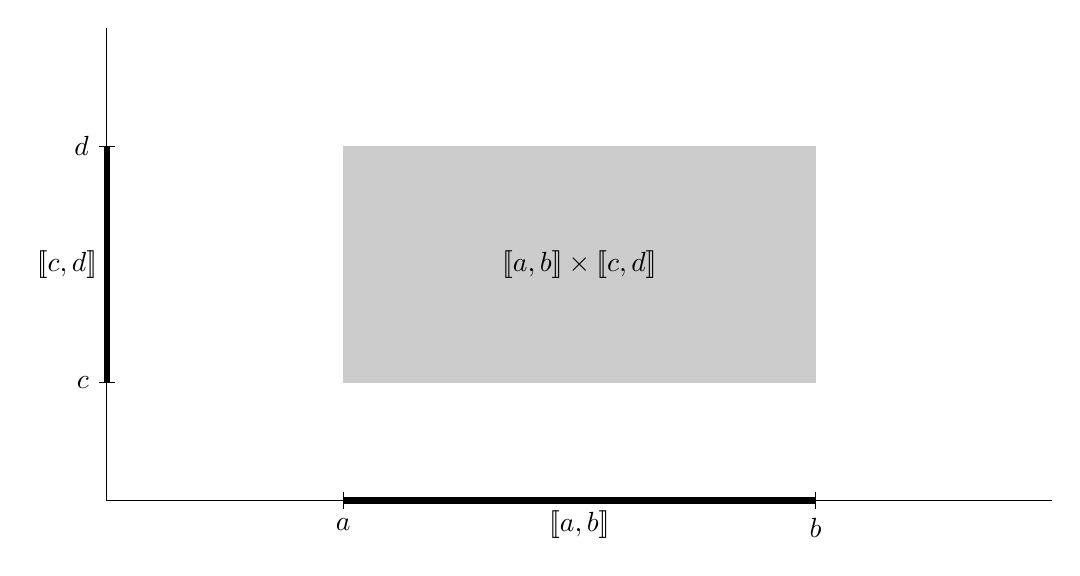
\begin{tikzpicture}[y=1.5cm, x=3cm]	
 	%axis
	\draw(0,0) -- coordinate (x axis mid) (4,0);
    	\draw (0,0) -- coordinate (y axis mid) (0,4);
    	
    	%ticks
    	\draw[fill] (1,1pt) rectangle (3,-1pt);    	
    	\draw (1, 3pt) -- (1, -3pt) node[anchor=north] {$a$};
    	\draw (3, 3pt) -- (3, -3pt) node[anchor=north] {$b$};
    	\draw (2, 0) node[anchor=north] {$[\![a,b]\!]$};
    	
    	\draw[fill] (1pt,1) rectangle (-1pt, 3);
    	\draw (3pt, 1) -- (-3pt, 1) node[anchor=east] {$c$};
    	\draw (3pt, 3) -- (-3pt, 3) node[anchor=east] {$d$};
    	\draw (0,2) node[anchor=east] {$[\![c,d]\!]$};
    	
    	\draw[fill, color=black!20] (1,1) rectangle (3,3);
    	\draw (2, 2) node {$[\![a,b]\!] \times [\![c,d]\!]$ };
	\end{tikzpicture}
	\caption[Cartesian product of two 1-rectangles] { 
		The Cartesian product of two positively oriented 1-rectangles $[\![a,b]\!]$ and $[\![c,d]\!]$ 
		is a positively oriented 2-rectangle.
	\label{fig:productofintervals}}
\end{figure}


There is no reason to stop here.
$[\![a,b]\!]\times [\![c,d]\!]$ is still a hybrid set, we can take its Cartesian product with another interval, say $[\![e,f]\!]$
to get a rectangular cuboid in $\mathbb{R}^3$.
We should note here that we do not distinguish between $((x,y),z)$ and $(x,(y,z))$
 but rather we treat both as different names for the ordered triple $(x,y,z)$.
That is, the Cartesian product is associative, and any difference in the brackets that arise:
\begin{equation*}
	\hset{ ((x, y), z)^{(m \cdot n)\cdot p} | x \in^m X, y \in^n Y, z \in^p Z }
	= X \times Y \times Z
	= \hset{ (x, (y, z)^{m \cdot (n\cdot p)} |  x \in^m X, y \in^n Y, z \in^p Z }
\end{equation*}
 
 
Although we will not be using them in this chapter, the objects resulting from iterated Cartesian product of intervals 
turn out to be quite useful.
We will call them $k$-rectangles.
A 1-dimensional (non-degenerate) oriented interval will be called a 1-rectangle.
A 2-dimensional rectangle will be called a 2-rectangle and a cuboid a 3-rectangle, and so on.

\begin{theorem}
	The Cartesian product of a $k$-rectangle in $\mathbb{R}^m$ (where, $k\leq m$) 
	and $\ell$-rectangle in $\mathbb{R}^n$ (again, $\ell \leq n$) 
	is a $(k+\ell)$-rectangle in $\mathbb{R}^{m+n}$.
\end{theorem}


For completeness we will also define a 0-rectangle as a hybrid set containing a single point with multiplicity $1$ or $-1$.
This allows us to embed $k$-rectangles in $\mathbb{R}^n$.
For example $[\![a,b]\!]_\mathbb{R} \times [\![c,d]\!]_\mathbb{R} \times \hset{e^1}$ is the product of two 1-rectangles
and a 0-rectangle and so it is a 2-rectangle.
But it was still a Cartesian product of 3 hybrid sets (each over $\mathbb{R}$) and so is a 2-rectangle in $\mathbb{R}^3$.
Specifically, it is the 2-rectangle $[\![a,b]\!] \times [\![c,d]\!]$ on the plane $z=e$.
This also illustrates the principle that given a $k$-rectangle in $\mathbb{R}^n$ where $n>k$ we can always find a $k$ 
dimensional subspace which also contains the rectangle.


Finally, one last note regarding $k$-rectangles before we return to the realm of symbolic linear algebra.
We will re-use the interval notation and allow for intervals between two vectors: $[\![\boldsymbol{a}, \boldsymbol{b}]\!]$.
But one should be careful to ``type-check'' when interpreting.
When $a$ and $b$ are real numbers then we continue to use the definition $[\![a,b]\!] = [a,b) \ominus [b,a)$.
However, when $\boldsymbol{a}$ and $\boldsymbol{b}$ are $n$-tuples (for example, coordinates in $\mathbb{R}^n$ 
then this is \emph{not} the oriented line interval, 
$[\boldsymbol{a}, \boldsymbol{b}) \ominus [\boldsymbol{b}, \boldsymbol{a})$
rather we define it as follows:

\begin{definition}
	Let $\boldsymbol{a} = (a_1, a_2, \ldots, a_n)$ and 
	$\boldsymbol{b} = (b_1, b_2, \ldots, b_n)$ be ordered $n$-tuples then we use the notation:
	\begin{equation}
		[\![ \boldsymbol{a}, \boldsymbol{b} ]\!] 
		= [\![a_1, b_1]\!] \times [\![a_2, b_2 ]\!] \times \ldots \times [\![a_n , b_n]\!]
	\end{equation}
\end{definition}

The dimension of $[\![ \boldsymbol{a}, \boldsymbol{b} ]\!]$ is equal to the number of indices where $a_i$ and $b_i$ are distinct.
For any $i$ where $a_i = b_i$, the corresponding term: $[\![ a_i, b_i ]\!]$ will be a hybrid set containing a single point, that is, a 0-rectangle.
The orientation of $[\![ \boldsymbol{a}, \boldsymbol{b} ]\!]$ is based on the number of negatively oriented intervals $[\![a_i,b_i]\!]$.
Should there be an odd number of indices $i$ such that $a_i > b_i$ then $[\![ \boldsymbol{a}, \boldsymbol{b} ]\!]$ will also be negatively oriented.
Otherwise, it will be positively oriented. 


For the remainder of this chapter, we will only be interested in matrices thought of as the space 
$\mathbb{N}_0 \times \mathbb{N}_0$.
Here there is only room for a single Cartesian product and so this notation will not be immediately useful. 
We will return to this discussion of higher dimension rectangles in Chapter 4 when investigating integration.




%%%%%%%%%%%%%%%%%%%%%%%%%%%%%%%%%%%%%%%%%
% Matrix Addition
%%%%%%%%%%%%%%%%%%%%%%%%%%%%%%%%%%%%%%%%%
\section{Matrix Addition}


Now we will consider the addition of $2 \times 2$ block matrices $A$ and $B$ with overall dimensions $n \times m$ 
of the form:
\begin{equation*}
	A = \left[ \begin{array}{c|c} A_{11} & A_{12} \\ \hline A_{21} & A_{22} \end{array} \right]
	\;\;\;\;\; \text{and} \;\;\;\;\;
	B = \left[ \begin{array}{c|c} B_{11} & B_{12} \\ \hline B_{21} & B_{22} \end{array} \right]
\end{equation*}
Since these are block matrices then $A_{ij}$ and $B_{ij}$ are not entries but sub matrices themselves.
We shall assume that $A_{11}$ is a $(q \times r)$ matrix and $B_{11}$ is a $(s \times t)$ matrix.
The sum of $A$ and $B$ will also be a $n \times m$ matrix.
Our universe, $\mathcal{U}$ is therefore the the set of all indices in an $n \times m$ matrix:
\begin{equation*}
	\mathcal{U} 
		\;=\; [\![0,n)\!)_{\mathbb{N}_0} \times [\![0,m)\!)_{\mathbb{N}_0} 
		\;=\; \{ (i,j) \;|\; 0 \leq i < n \text{ and } 0 \leq j < m \text{ and } i,j \in \mathbb{N}_0 \} 
\end{equation*}


First we must convert $A$ and $B$ to hybrid function notation. 
We will use $\mathcal{A}_{ij}$ an $\mathcal{B}_{ij}$ to respectively denote the regions for which 
$A_{11}$ and $B_{ij}$ are defined.
Explicitly,
\begin{align*}
	&\mathcal{A}_{11} = [\![0,q)\!) \times [\![0,r)\!) &
	\mathcal{A}_{12} = [\![0,q)\!) \times [\![r,m)\!)\;\; &
	\mathcal{A}_{21} = [\![q,n)\!) \times [\![0,r)\!) &
	\mathcal{A}_{22} = [\![q,n)\!) \times [\![r,m)\!) \\
	&\mathcal{B}_{11} = [\![0,s)\!) \times [\![0,t)\!) &
	\mathcal{B}_{12} = [\![0,s)\!) \times [\![t,m)\!)\;\; &
	\mathcal{B}_{21} = [\![s,n)\!) \times [\![0,t)\!) &
	\mathcal{B}_{22} = [\![s,n)\!) \times [\![t,m)\!)
\end{align*}
Which will allow us to rewrite $A$ and $B$ as:
\begin{align*}
	A &= A_{11}^{\mathcal{A}_{11}} \oplus 
		A_{12}^{\mathcal{A}_{12}} \oplus 
		A_{21}^{\mathcal{A}_{21}} \oplus 
		A_{22}^{\mathcal{A}_{22}} \\
	B &= B_{11}^{\mathcal{B}_{11}} \oplus 
		B_{12}^{\mathcal{B}_{12}} \oplus 
		B_{21}^{\mathcal{B}_{21}} \oplus 
		B_{22}^{\mathcal{B}_{22}} 
\end{align*}


Depending on the relation of $q$ with $s$ and $r$ with $t$ the regions in the sum of $A$ and $B$ may vary.
In Figure~\ref{MatAdditionPermutations}, the shapes of block matrices that can arise are shown.
Intuitively, the approach we will take is to not concern ourselves with all possible cases that \emph{could} arise but to just
choose one ordering.
If this ordering is wrong, then the hybrid function multiplicities will handle cancellations to yield the correct expression regardless.


Since there are 4 partitions in $A$ and 4 partitions in $B$, we only require 7 pieces to form a common refinement.
To this refinement for, we follow the same method as used previously:
\begin{equation}
	\label{eqn:2x2CommonRefinement}
	\Big\{ \;
		\mathcal{A}_{11}, \; \mathcal{A}_{12}, \;  \mathcal{A}_{21}, \;
		\mathcal{B}_{11}, \; \mathcal{B}_{12}, \; \mathcal{B}_{21}, \; \mathcal{P} 
	\; \Big\}
\end{equation}
with $\mathcal{P}$ is defined as,
\begin{equation*}
	\mathcal{P} = \mathcal{U} 
		\ominus \left( \mathcal{A}_{11} \oplus \mathcal{A}_{12} \oplus \mathcal{A}_{21} \oplus
				\mathcal{B}_{11} \oplus \mathcal{B}_{12} \oplus \mathcal{B}_{21} \right)
\end{equation*}
Clearly we can still express $\mathcal{A}_{22}$ using only the terms from the common refinement by:
\begin{align*}
	\mathcal{A}_{22} 
		&= \mathcal{U} \ominus (\mathcal{A}_{11} \oplus \mathcal{A}_{12} \oplus \mathcal{A}_{21}) \\[-0.5em]
		& = \mathcal{U} \ominus (\mathcal{A}_{11} \oplus \mathcal{A}_{12} \oplus \mathcal{A}_{21} 
			\oplus \mathcal{B}_{11} \oplus \mathcal{B}_{12} \oplus \mathcal{B}_{21}) 
			\oplus \mathcal{B}_{11} \oplus \mathcal{B}_{12} \oplus \mathcal{B}_{21}\\[-0.5em]
		&= \mathcal{P} \oplus \mathcal{B}_{11} \oplus \mathcal{B}_{12} \oplus \mathcal{B}_{21}
\end{align*}
Similarly $\mathcal{B}_{22}$ can be represented as $\mathcal{B}_{22} = \mathcal{P} \oplus \mathcal{A}_{11} \oplus \mathcal{A}_{12} \oplus \mathcal{A}_{21}$
and $\mathcal{U}$ as the sum of all 7 regions, 
$\mathcal{U} = 	\mathcal{A}_{11} \oplus \mathcal{A}_{12} \oplus \mathcal{A}_{21} \oplus 
				\mathcal{B}_{11} \oplus \mathcal{B}_{12} \oplus \mathcal{B}_{21} \oplus \mathcal{P}$.
Thus $A$ and $B$ can be rewritten using this new generalized partition as:
\begin{align*}
	A &= A_{11}^{\mathcal{A}_{11}} \oplus 
		A_{12}^{\mathcal{A}_{12}} \oplus 
		A_{21}^{\mathcal{A}_{21}} \oplus 
		A_{22}^{\mathcal{P} \oplus \mathcal{B}_{11} \oplus \mathcal{B}_{12} \oplus \mathcal{B}_{21}} \\
	B &= B_{11}^{\mathcal{B}_{11}} \oplus 
		B_{12}^{\mathcal{B}_{12}} \oplus 
		B_{21}^{\mathcal{B}_{21}} \oplus 
		B_{22}^{\mathcal{P} \oplus \mathcal{A}_{11} \oplus \mathcal{A}_{12} \oplus \mathcal{A}_{21}} 
\end{align*}

And addition becomes straightforward. 
We add functions for terms over corresponding regions.
Since we are using \emph{generalized partitions}, not traditional partitions we cannot guarantee disjointness.
As such we must also apply a $+$-reduction after summing each matching pair:
\begin{align*}
	(A+B) = \R[+] & \left(  (A_{11}+B_{22})^{\mathcal{A}_{11}} \oplus 
		(A_{12} + B_{22})^{\mathcal{A}_{12}} \oplus 
		(A_{21} + B_{22})^{\mathcal{A}_{21}} \right. \\[-0.5em] &\oplus 
		(A_{22} + B_{11})^{\mathcal{B}_{11}} \oplus 
		(A_{22} + B_{12})^{\mathcal{B}_{12}} \oplus 
		(A_{22} + B_{21})^{\mathcal{B}_{21}} \\[-0.5em] &\oplus
		\left.(A_{22} + B_{22})^{\mathcal{P}} \right)
\end{align*}


\subsection{Example: \emph{Evaluation at points}} 
We will now demonstrate evaluating this expression.
Let us assume a point $(i,j)$ exists in the region $\mathcal{A}_{11} \cap \mathcal{B}_{12}$.
That is, $0 \leq i < \min(q,s)$ and $t \leq j < r$. 
Evaluating each of the hybrid sets from (\ref{eqn:2x2CommonRefinement}) we find that only three have 
non-zero multiplicities: $\mathcal{A}_{11}(i,j)=1$, $\mathcal{B}_{12}=1$ and 
$\mathcal{P}(i,j)=1-(1+0+0+0+1+0)=-1$.
After removing all zero terms, this yields:
\begin{align*}
	(A+B)(i,j) &= \R[+]  \left(  (A_{11}+B_{22})^{1} \oplus 
		(A_{22} + B_{12})^{1} \oplus 
		(A_{22} + B_{22})^{-1} \right)\\
		&= \left(A_{11}+B_{22}) + (A_{22} + B_{12}) - (A_{22} + B_{22}\right)(i,j)\\
		&= (A_{11}+B_{12})(i,j)
\end{align*}

As a second example assume $(i,j) \in \mathcal{A}_{22} \cap \mathcal{B}_{12}$.
Then we find there is only one partition with non-zero multiplicity.
Clearly $\mathcal{B}_{12} = 1$ but $\mathcal{A}_{22} \notin$(\ref{eqn:2x2CommonRefinement}).
Calculating the multiplicity of $\mathcal{P}$ also yields $1-(0+0+0+0+1+0) = 0$.
Very simply:
\begin{align*}
	(A+B)(i,j) &= \R[+]  \left(  (A_{22}+B_{12})^{1} \right)(i,j)\\
		&=(A_{22}+B_{12})(i,j)
\end{align*}


\subsection{Addition with Larger Block Matrices}
This method extends easily from addition of two $2\times 2$ block matrices to arbitrary addition of block matrices.
If we consider (\emph{conformable}) $k \times \ell$ and $n \times m$ block matrices $A$ and $B$ respectively of the form:

\begin{equation*}
	A = \begin{bmatrix}
		A_{11} & \ldots & A_{1\ell}\\
		\vdots & & \vdots \\
		A_{k1} & \ldots & A_{k\ell}	
	\end{bmatrix}
	\;\;\;\;\;
	\text{ and }
	\;\;\;\;\;
	B = \begin{bmatrix}
		B_{11} & \ldots & B_{1m}\\
		\vdots & & \vdots \\
		B_{n1} & \ldots & B_{nm}	
	\end{bmatrix}
\end{equation*}

For matrices to be conformable for additon they must have the same dimensions.
So we can partition the rows of $A$ by the strictly increasing sequence $\{q_i\}_{i=0}^k$ and 
the columns by $\{r_j \}_{j=0}^\ell$.
Similarly for $B$ we partition the rows by $\{s_i\}_{i=0}^n$ and the columns by $\{t_j\}_{j=0}^m$.
With the additional constraints that ${q_0 = r_0 = s_0 = t_0 = 0}$ and $q_k = s_n$ and $r_\ell = t_m$.
Each $A_{ij}$ and $B_{ij}$ is defined over a rectangular region $\mathcal{A}_{ij}$ and $\mathcal{B}_{ij}$:
 \begin{equation*}
	\mathcal{A}_{ij} = [\![q_{i-1}, q_i )\!) \times [\![ r_{j-1}, r_{j} )\!)
	\;\;\;\;\;
	\mathcal{B}_{ij} = [\![s_{i-1}, s_i )\!) \times [\![ t_{j-1}, t_{j} )\!)
\end{equation*}
which gives the expression:
\begin{equation}
	(A+B) = \R[+] \left( 
		\left( \bigoplus_{(i,j) \neq (n,m)} (A_{ij} + B_{nm})^{\mathcal{A}_{ij}} \right) \oplus
		\left( \bigoplus_{(i,j) \neq (n,m)} (A_{nm} + B_{ij})^{\mathcal{B}_{ij}} \right) \oplus
			(A_{nm} + B_{nm})^{\mathcal{P}} 
	\right)
\end{equation}




%%%%%%%%%%%%%%%%%%%%%%%%%%%%%%%%%%%%%%%%%
% Matrix Multiplication
%
% q = k1, r = q2, s = ell1, t=ell2
%%%%%%%%%%%%%%%%%%%%%%%%%%%%%%%%%%%%%%%%%
\section{Matrix Multiplication}


Next we will consider the product of symbolic block matrices.
Again, we will assume $2 \times 2$ block matrices $A$ and $B$.
However for these matrices to be conformable for multiplication they must be  $n \times m$ and $m \times p$ rather than
the same size as was required for addition.
\begin{equation}
	A = \begin{bmatrix} A_{11} & A_{12} \\ A_{21} & A_{22} \end{bmatrix}
	\;\;\;\;\; \text{and} \;\;\;\;\;
	B = \begin{bmatrix} B_{11} & B_{12} \\ B_{21} & B_{22} \end{bmatrix}
\end{equation}
Where $A_{11}$ is a $q \times r$ matrix and $B_{11}$ is a $s \times t$ matrix.
Note that $0 \leq r , s \leq m$ but the ordering of $r$ and $s$ is unknown.


In the simplest case, $r=s$, four regions will arise each with simple closed expressions. 
\begin{equation}
	AB = \begin{bmatrix}
		\left( A_{11}B_{11}+A_{12}B_{21} \right) & \left( A_{11}B_{12}+A_{12}B_{22} \right) \\ 
		\left( A_{21}B_{11}+A_{22}B_{21} \right) & \left( A_{21}B_{12}+A_{22}B_{22} \right)
	\end{bmatrix}
\end{equation}
One should notice the similarity between this and multiplication of simple $2 \times 2$ matrices.
If we consider only the top-left block, since $r=s$ then the $(q \times r)$ matrix $A_{11}$ and the 
$(s \times t)$ matrix $B_{11}$ are conformable.
As are the $(q \times m-r)$ matrix $A_{12}$ and the $(m-s \times t)$ matrix $B_{21}$.
Both products will result in a $q \times t$ matrix which are conformable for addition.
Thus the term $A_{11}B_{11} + A_{12}B_{21}$ is a $q \times t$ block. 


If $r \neq s$ then one approach would be to partition $A$ into a $2 \times 3$ block matrix 
split along the vertical lines $r$ and $s$ and the horizontal line $q$.
And split $B$ into a $3 \times 2$ block matrix split along the vertical line $t$  and the horizontal lines $r$ and $s$:
Depending on the relative ordering of $r$ and $s$ this may cause different blocks to be split.
If $s < r$ then $A_{11}$ and $A_{21}$ will be split into blocks with columns from 0 to $s$ and then from $s$ to $r$
while $B_{21}$ and $B_{22}$ would be split into blocks with rows from $s$ to $r$ and from $r$ to $m$.
\begin{equation*}
	A= \left[ \begin{array}{cc|c}
			A_{11}^{(1)} & A_{11}^{(2)} & A_{12}^{} \\ 
			\hline
			A_{21}^{(1)} & A_{21}^{(2)} & A_{22}^{}
		\end{array} \right]
	\;\;\;\;\;\text{and}\;\;\;\;\;
	B = \left[ \begin{array}{c|c}
			B_{11}^{} & B_{12}^{} \\
			\hline
			B_{21}^{(1)} & B_{22}^{(1)} \\
			B_{21}^{(2)} & B_{22}^{(2)} 
		\end{array} \right]
\end{equation*}


The resulting product is still a $2 \times 2$ matrix.
Additionally, each block is still the same size; the first block in the top-left is still $q \times t$.
However each block is now the sum of three block products:
\begin{equation*}
	AB 	= 	\begin{bmatrix}
				\left( A_{11}^{(1)}B_{11}^{}+ A_{11}^{(2)}B_{21}^{(1)} + A_{12}^{}B_{21}^{(2)} \right) & 
				\left( A_{11}^{(1)}B_{12}^{}+ A_{11}^{(2)}B_{22}^{(1)} + A_{12}^{}B_{22}^{(2)} \right) \\
				\left( A_{21}^{(1)}B_{11}^{}+ A_{21}^{(2)}B_{21}^{(1)} + A_{22}^{}B_{21}^{(2)} \right) & 
				\left( A_{21}^{(1)}B_{12}^{}+ A_{21}^{(2)}B_{22}^{(1)} + A_{22}^{}B_{22}^{(2)} \right) 
			\end{bmatrix}
\end{equation*}
On the other hand, if $r < s$ then $A_{12}$ and $A_{22}$ will be the blocks split vertically while $B_{11}$ and $B_{12}$
will be split horizontally. 
In turn, this leads to a different expression for the product of $A$ and $B$.
In a now familiar, pattern we can use hybrid functions to give a single expression 
to deal with all permutations simultaneously.


First we shall refer to the product $AB$ by the block matrix $C$:
\begin{equation}
	AB = C = \begin{bmatrix} C_{11} & C_{12} \\ C_{21} & C_{22} \end{bmatrix}
\end{equation}
$C$ is an $n \times p$ matrix as determined by the sizes of $A$ and $B$ and $C_{11}$ is a $q \times t$ sub-matrix.
This leaves $C_{12}$, $C_{21}$ and $C_{22}$ to be $q \times (p-t)$, $(n-q) \times t$ and $(n-q) \times (p-t)$ respectively.
We will partition all three matrices along the axes $0.. n$, $0..p$ and $0..m$ into the oriented intervals:
\begin{align*}
	N_1 	&= [\![0, q)\!) 	& N_2 	&= [\![q, n)\!) 	\\
	P_1 	&= [\![0, t)\!) 	& P_2 	&= [\![t, p)\!) 	\\
	M_1 	&= [\![0, r)\!) 	& M_2 	&= [\![r, s)\!) 	& M_3 	&= [\![s, m)\!)
\end{align*}


Assumption is too strong a word, but these partitions follow the \emph{guess} that $r<s$.
So we will be constructing expressions with this in mind. 
If we chose incorrectly, then we plan to use the negative orientation of $M_2$ to correct our expression.
Using these intervals, we can now rewrite our matrices inline as:
\begin{align}
	A & =	A_{11}^{N_1 \times M_1} \oplus A_{12}^{N_1 \times (M_2 \oplus M_3)} \oplus 
			A_{21}^{N_2 \times M_1} \oplus A_{22}^{N_2 \times (M_2 \oplus M_3)} \\
	B & =	B_{11}^{(M_1 \oplus M_2) \times P_1} \oplus B_{12}^{(M_1 \oplus M_2) \times P_2} \oplus 
			B_{21}^{M_3 \times P_1} \oplus B_{12}^{M_3 \times P_2}\\
	\label{eqn:2x2multiplicationblocks}
	C & =	C_{11}^{N_1 \times P_1} \oplus C_{12}^{N_1 \times P_2} \oplus
			C_{21}^{N_2 \times P_1} \oplus C_{22}^{N_2 \times P_2}
\end{align}
It should be noted here that $\oplus$ is still the point-wise sum of hybrid functions.
It should not be confused with the direct sum nor the Kronecker sum of matrices which both use the same $\oplus$ operator.
The $\times$ operator refers to the Cartesian product of intervals. 


For $i,j \in \{ 1,2 \}$ the terms of $C$ are given by.
\begin{align}
	\label{eqn:2x2multiplication}
	C_{i,j}^{N_i1 \times P_j} (x,y) = \sum_{M} \R[\times]  
		&\left( \;\;
			\left. 	A_{i,1}^{N_1 \times M_1}	\right|_{X=x} \;\oplus\;
			\left.	B_{1,j}^{M_1 \times P_1}	\right|_{Y=y} 
		\right.  \notag \\
	 	&\oplus
	 		\left.	A_{i,2}^{N_1 \times M_2}	\right|_{X=x} \;\oplus\;
			\left. 	B_{1,j}^{M_2 \times P_1}	\right|_{Y=y} 
		\notag \\
		&\oplus\left.
			\left.	A_{i,2}^{N_1 \times M_3}	\right|_{X=x} \;\oplus\;
			\left. 	B_{2,j}^{M_3 \times P_1}	\right|_{Y=y}
		\;\;\right)
\end{align}


There is some new notation here so let us unpack it.
Recall that we are taking the approach that matrices are simply functions defined on $\mathbb{N} \times \mathbb{N}$.
As a function we can take a restriction of a matrix to a set of indices.
In the above, we use $X$ and $Y$ to denote the row and column indexing respectively.
For example with the matrix $M$, given below $M|_{X=0}$ and $M_{Y=0}$ would be as follows:
\begin{align*}
	M &= \begin{bmatrix}
		M[0,0] 	& \ldots 	& M[0,n] \\
		\vdots 	& 		& \vdots \\
		M[m,0]	& \ldots & M[m,n]
	\end{bmatrix} &
	M|_{X=0} &= \begin{bmatrix}
		M[0,0] & \ldots & M[0,n]
	\end{bmatrix} &
	M|_{Y=0} &= \begin{bmatrix}
		M[0,0] \\ \vdots \\ M[m,0]
	\end{bmatrix}
\end{align*}


But this is more powerful than just simple evaluation.
We are selecting not a fixed axis as $(x,y)$ is the input to our function.
And so for a matrix $M|_{X=x}$ or $M|_{Y=y}$ we transform $M:X\times Y \to Z$
to the curried $M|_{X=i}:Y \to ( X \to Z)$ or $M|_{Y=j}:X \to (Y \to Z)$.
Within the context of \ref{eqn:2x2multiplication}, this transforms the blocks of $A$ into horizontal vector slices 
and $B$ into vertical slices.


Ignoring the differences in transposition, when thought of as functions these functions both map from $M$ 
(the common axis of $A$ and $B$) to functions with a common range.
And so we have the pointwise sum of terms of the forms $m \mapsto ( x \mapsto A[x][m] )$ and 
$m \mapsto (y \mapsto B[m][y])$.
The work of multiplying matching $A[x][m]$ with $B[m][y]$ is handled by the $\R[\times]$.
This leaves us with the product of two functions with different domains, but common range:
\begin{equation*}
	 ( x \mapsto A[x][m] )\times (y \mapsto B[m][y]) 
	 = (x,y) \mapsto A[x][m] \times B[m][y]
\end{equation*}


Finally, we have the sum over $M$.
If $A$ and $B$ are matrices over a field $F$ then the \mbox{$\times$-reduction} 
yields a function $M \to (N \times P \to F)$.
Summing over the set $M$ leaves us with a function $(N \times P \to F)$ which agrees (at least by object type) 
with our expectations for $C$.
The familiar structure of summing over a product suggest correctness when $\big\{ M_1, M_2, M_3 \big\}$ 
is a strict partition of $M$ (that is, when $r \leq s$).
Despite the mental hurdles of say a $2 \times (-3)$ matrix, it continues to hold for general partitions as well.





%%%%%%%%%%%%%%%%%%%%%%%%%%%%%%%%%%%%%%%%%
% Multiplication Example
%%%%%%%%%%%%%%%%%%%%%%%%%%%%%%%%%%%%%%%%%
\subsection{Example: \emph{Matrix Multiplication Concretely}}


We will consider the product of two block matrices $Q$ and $R$.
For this example, to better differentiate between blocks, 
we will change our notation slightly and give each block a distinct letter names: 
$A,B,C,D$ for the blocks of $Q$ and $E,F,G,H$ for the blocks of $R$.
\begin{equation*}
	Q = \left[ \begin{array}{cc|c}
		a_1 & a_2 & b_1 \\
		a_3 & a_4 & b_2 \\
		\hline
		c_1 & c_2 & d_1 \\
		c_3 & c_4 & d_2
	\end{array} \right]
	\;\;\;\;\; \text{and} \;\;\;\;\;
	R = \left[ \begin{array}{c|cccc}
		e_1 & f_1 & f_2 & f_3 & f_4 \\
		\hline
		g_1 & h_1 & h_2 & h_3 & h_4 \\
		g_2 & h_5 & h_6 & h_7 & h_8
	\end{array} \right]
\end{equation*}


We will again use $M$, $N$ and $P$ for the sets of indices.
As $4 \times 3$ and $3\times 5$ matrices, we have $M = [\![0,3]\!]$, $N=[\![0,2]\!]$ and $P=[\![0,4]\!]$.
To align with the blocks of $Q$ and $R$, each of these sets is partitioned as follow:
\begin{align*}
	N_1 	&= [\![0, 1]\!] 	& N_2 	&= [\![2, 3]\!] 	\\
	P_1 	&= [\![0]\!] = \hset{0^{+1}}		& P_2 	&= [\![1, 4]\!] 	\\
	M_1 	&= [\![0, 1]\!] 	& M_2 	&= (\!(1)\!) = \hset{1^{-1}} 	& M_3 	&= [\![1, 2]\!]
\end{align*}
We should note here that our guess was wrong; $M_2$ is negatively oriented!
Although we could have constructed two expressions to handle this case as well, this will not be necessary.
We can continue as if nothing is wrong, and the hybrid function structure will take care of cancellations.


We can still write $Q$  and $R$ as:
\begin{align*}
	Q &= A^{N_1 \times M_1} \oplus 
		B^{N_1 \times (M_2 \oplus M_3)} \oplus
		C^{N_2 \times M_1} \oplus
		D^{N_2 \times (M_2 \oplus M_3)}\\
	R &= E^{(M_1 \oplus M_2) \times P_1} \oplus
		F^{(M_1 \oplus M_2) \times P_2} \oplus
		G^{M_3 \times P_1} \oplus
		H^{M_3 \times P_2}	
\end{align*}
The only difference is that originally the sum $(M_2 \oplus M_3) = \{ 2 \}$ was intended to \emph{extend} $M_3$.
When $M_2$ is negative, it is a set of indices which is \emph{smaller} than the $M_3 = \{ 1,2 \}$ we started with.
Similarly, in the expression for $R$, $(M_1 \oplus M_2)$ is smaller than $M_1$.
We will use $S$ to denote the product $QR$ which is still another $2\times 2$ block matrix by the same construction 
as (\ref{eqn:2x2multiplicationblocks}):
\begin{equation*}
	S = Q \cdot R  =
		\begin{bmatrix} S_1 & S_2 \\ S_3 & S_4 \end{bmatrix} =
		 {S_1}^{N_1 \times P_1} \oplus
		 {S_2}^{N_1 \times P_2} \oplus
		 {S_3}^{N_2 \times P_1} \oplus
		 {S_4}^{N_2 \times P_2}
\end{equation*}


Let us compute one of these blocks: $S_1$.
\begin{align*}
	{S_1}^{N_1 \times P_1}(i,j) = \sum_{m \in M ?} \R[\times]  &\left( 
			\left. A^{N_1 \times M_1}\right|_{X=i} \oplus
			\left. E^{M_1 \times P_1}\right|_{Y=j} \oplus \right.\\
			&\;\left. B^{N_1 \times M_2}\right|_{X=i} \oplus
			\left. E^{M_2 \times P_1}\right|_{Y=j} \oplus\\ 
			&\;\left. \left. B^{N_1 \times M_3}\right|_{X=i} \oplus
			\left. G^{M_3 \times P_1}\right|_{Y=j}
	\right)
\end{align*}
As this is a small example our curried functions only range over $\{ 0, 1, 2 \}$.
This is a small enough domain to express each of the functions as a set of point-wise mappings.
So let's expand out each of our terms as formal \emph{hybrid sets} 
(recall a hybrid function is a special hybrid set of ordered pairs):
\begin{align*}
	\sum_{m \in M ?} \R[\times] \bigg( 
		&\;\;\hset{
			\left( 0 \mapsto 
				\left[\begin{smallmatrix}\vphantom{b}a_1 \\ \vphantom{b}a_3 \end{smallmatrix}\right]
			\right)^{+1}, \;
			\left( 1 \mapsto 
				\left[\begin{smallmatrix}\vphantom{b}a_2 \\ \vphantom{b}a_4 \end{smallmatrix}\right]
			\right)^{+1}}  
		&&\oplus \hset{ 
			\left( 0 \mapsto [ e_1 ] \right)^{+1}, \;
			\left( 1 \mapsto [e_\bot] \right)^{+1}} \\ 
		&\oplus \hset{ 
			\left( 1 \mapsto \left[\begin{smallmatrix} b_\bot \\ b_\bot \end{smallmatrix}\right] \right)^{-1} }
		&&\oplus \hset{ 
			\left( 1 \mapsto [ e_\bot ] \right)^{-1} } \\
		&\oplus \hset{
			\left( 1 \mapsto \left[ \begin{smallmatrix} b_\bot \\ b_\bot \end{smallmatrix} \right] \right)^{+1}, \;
			\left( 2 \mapsto \left[ \begin{smallmatrix} b_1 \\ b_2 \end{smallmatrix}\right] \right)^{+1} }
		&&\oplus \hset{
			\left( 2 \mapsto [ g_1 ] \right)^{+1},\; 
			\left( 2 \mapsto [ g_2 ] \right)^{+1}}	\bigg)
\end{align*}


We are using $e_\bot$ and $b_\bot$ here to represent that the functions $E$ and $B$ are undefined for these points.
In reality, we would simply not even attempt to evaluate $B|_{X=x}(1)$ or $E|_{Y=y}(1)$ as the functions are undefined.
These points are actually contained in the $A$ and $G$ blocks, once again we must delay evaluation with pseudo-functions.


Applying the $\times$-reduction $\R[\times]$, we group terms by their input value (e.g. $1 \mapsto x$ with $1 \mapsto y$) 
and flatten using the multiplicity to repeat or invert the $\times$ operator.
In this case, we are dealing only with multiplicities of $+1$ and $-1$ which correspond with multiplication and ``division''.
This is not true division, as $0 \times^{-1} 0 = 1$ without fear of division by zero.
Otherwise for non-zero operands, $\times^{-1}$ agrees with the normal understanding of division.
This is made possible by working with multiplication as a \emph{group} rather than as a \emph{ring}
and so we are not worried about making multiplication ``play nice'' with addition.
Doing this yields:
\begin{align*}
	\sum_{M_1 \oplus M_2 \oplus M_3}
		& \left\{\!\left|\; \left(0 \mapsto 
			\left[\begin{smallmatrix}\vphantom{b}a_1 \\ \vphantom{b}a_3 \end{smallmatrix}\right] \times^{+1} 
			[e_1] \right), \right.\right.\\
		&\;\;\;\left(1 \mapsto 
			\left[\begin{smallmatrix}\vphantom{b}a_2 \\ \vphantom{b}a_4 \end{smallmatrix}\right] \times^{+1}
			[e_\bot] \times^{-1}
			\left[\begin{smallmatrix} b_\bot \\ b_\bot \end{smallmatrix}\right] \times^{-1}
			[ e_\bot ]\times^{+1}
			\left[ \begin{smallmatrix} b_\bot \\ b_\bot \end{smallmatrix} \right] \right)
			[ g_1 ],\\
		&\;\;\left.\left.\left(2 \mapsto 
			\left[ \begin{smallmatrix} b_1 \\ b_2 \end{smallmatrix}\right]\times^{+1}
			[ g_2 ] \right) \; \right|\!\right\}
\end{align*}


After some cancellations in the second term, we evaluate $\times^{+1}$ as matrix multiplication and sum over all of $M$:
\begin{equation*}
	{S_1}^{N_1 \times P_1} =
			\begin{bmatrix}\vphantom{b}a_1 \\ \vphantom{b}a_3 \end{bmatrix}
			[e_1]
		+ 	\begin{bmatrix}\vphantom{b}a_2 \\ \vphantom{b}a_4 \end{bmatrix}
			[g_1]
		+	\begin{bmatrix} b_1 \\ b_2 \end{bmatrix}
			[ g_2 ]
		=  \begin{bmatrix}a_1e_1+a_2g_1+b_2g_2\\ a_3e_1+a_4b_1+b_2g_2\end{bmatrix}
\end{equation*}
As expected we have a $|N_1| \times |P_1| = (2 \times 1)$ matrix which will form the upper left block of $S$.
Ignoring the block structure of $Q$ and $R$ and performing normal matrix multiplication, we also find that these values 
agree with $S[0,0]$ and $S[1,0]$.
Computations for the blocks $S_2$, $S_3$ and $S_4$ are performed identically yielding blocks of varying sizes.
Together, theses blocks form a strict partitioning of $S$ as a $2\times 2$ block matrix.







%%%%%%%%%%%%%%%%%%%%%%%%%%%%%%%%%%%%%%%%%
% Larger multiplication
%%%%%%%%%%%%%%%%%%%%%%%%%%%%%%%%%%%%%%%%%
\subsection{Multiplication with Larger Block Matrices}

The most difficult part of extending block matrix multiplication to larger block matrices turns out to be the number of 
variables needed.
Once again we will use $N_i$ to divide the rows of blocks in $A$ and $P_j$ to divide the block columns of $B$.
\begin{align*}
	A &= \bigoplus_{i \in [\![1,I]\!]} \bigoplus_{k \in [\![1,K]\!]} A_{i,k}^{N_i \times M_k}&
	B &= \bigoplus_{k' \in [\![1,K']\!]} \bigoplus_{j \in [\![1,J]\!]} B_{k',j}^{M'_{k'} \times P_j}
\end{align*}
And as before the blocks of $C$ will be $N_i \times P_j$
\begin{equation}
	C = \bigoplus_{i \in [\![1,I]\!]} \bigoplus_{j \in [\![1,J]\!]} C_{i,j}^{N_i \times P_j}
\end{equation}
Where each $C_{i,j}$ is defined as:
\begin{equation}
	C_{i,j} = 	\left(\sum_{k \in [\![1,K)\!)} A_{i,k}^{N_i \times M_k} B_{K',j}^{M_k \times P_j} \right)+ 
				\left(\sum_{k' \in [\![1,K')\!)} A_{i,K}^{N_i \times M_{k'}} B_{k',j}^{M_{k'} \times P_j} \right)+ 
				A_{i,K}^{N_i \times R} B_{K',j}^{R \times P_j}
\end{equation}
Again we must find a common refinement of $\{M_k\}_{k=1}^K$ and $\{M'_{k'}\}_{k'=1}^{K'}$.
We will use the same construction as earlier taking the first $K-1$ and $K'-1$ pieces respectively and then forming one 
``remainder'' piece, which here is 
$R =U \ominus \left( \bigoplus_{k \in [\![1,K)\!)} M_k \oplus \bigoplus_{k' \in [\![1,K')\!)} M'_{k'}\right)$





